\documentclass[11pt,reqno]{article}
\usepackage{amsthm, amsmath, amsfonts, amssymb, amscd, mathtools, youngtab, euscript, mathrsfs, verbatim, enumerate, multicol, multirow, bbding, color, babel, esint, geometry, tikz, tikz-cd, tikz-3dplot, tkz-graph, array, enumitem, thm-restate, thmtools, datetime, graphicx, tensor, braket, slashed, standalone, pgfplots, ytableau, subfigure, wrapfig, dsfont, setspace, wasysym, pifont, float, rotating, adjustbox, pict2e,array, physics, pgfplots}
\usepackage[colorlinks=true,linktocpage=true,linkcolor=DarkBlue,citecolor=DarkBlue,urlcolor=DarkBlue]{hyperref}
\usepackage{amsmath}
\usepackage[T1]{fontenc}
\usepackage[utf8]{inputenc}

\begin{document}

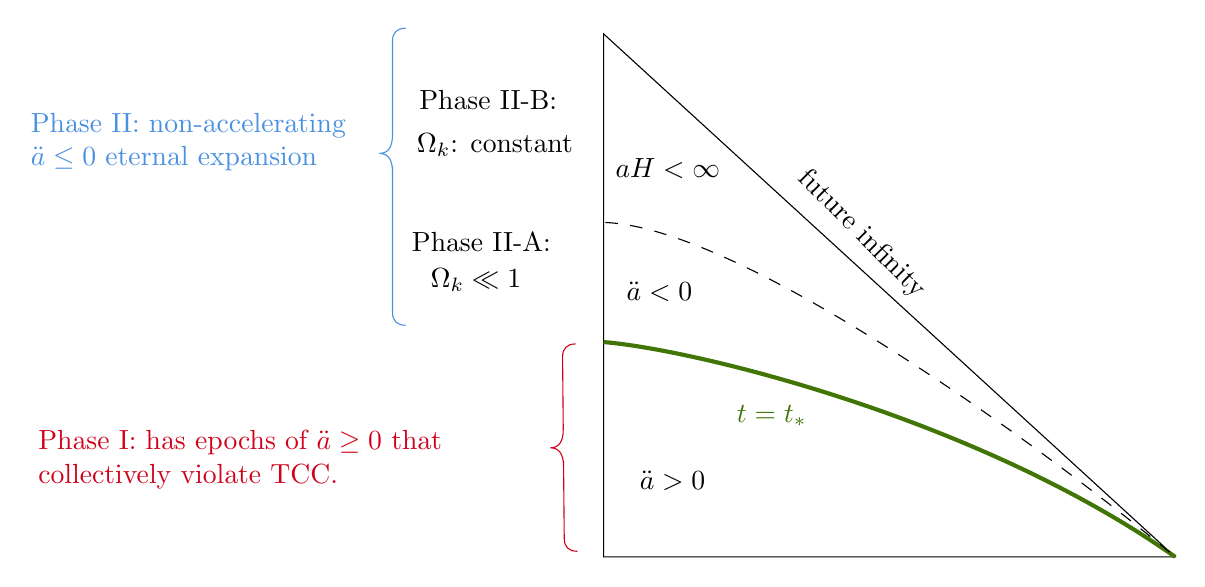
\begin{tikzpicture}[x=0.75pt,y=0.75pt,yscale=-0.9,xscale=0.9]

\draw   (316,10) -- (622,290) -- (316,290) -- cycle ;
\draw [color={rgb, 255:red, 65; green, 117; blue, 5 }  ,draw opacity=1 ][line width=1.5]    (316,175) .. controls (365,179) and (517,216) .. (622,290) ;
\draw  [color={rgb, 255:red, 208; green, 2; blue, 27 }  ,draw opacity=1 ] (301,176) .. controls (296.33,176.04) and (294.02,178.39) .. (294.06,183.06) -- (294.41,221.56) .. controls (294.47,228.23) and (292.17,231.58) .. (287.5,231.63) .. controls (292.17,231.58) and (294.53,234.89) .. (294.59,241.56)(294.57,238.56) -- (294.94,280.06) .. controls (294.99,284.73) and (297.34,287.04) .. (302.01,287) ;
\begin{scope}[shift={(12, 0)}]
\draw  [color={rgb, 255:red, 74; green, 144; blue, 226 }  ,draw opacity=1 ] (198,7) .. controls (193.33,7) and (191,9.33) .. (191,14) -- (191,64) .. controls (191,70.67) and (188.67,74) .. (184,74) .. controls (188.67,74) and (191,77.33) .. (191,84)(191,81) -- (191,159) .. controls (191,163.67) and (193.33,166) .. (198,166) ;
\end{scope}
\draw  [dash pattern={on 4.5pt off 4.5pt}]  (317,111) .. controls (392,114) and (556,235) .. (622,290) ;

% Text Node
\draw (426.75,78.73) node [anchor=north west][inner sep=0.75pt]  [rotate=-45] [align=left] {future infinity};
% Text Node
\draw (8,51) node [anchor=north west][inner sep=0.75pt]  [color={rgb, 255:red, 74; green, 144; blue, 226 }  ,opacity=1 ] [align=left] {Phase II: non-accelerating\\$\displaystyle \ddot{a} \leq 0$ eternal expansion};
% Text Node
\draw (12,221) node [anchor=north west][inner sep=0.75pt]  [color={rgb, 255:red, 208; green, 2; blue, 27 }  ,opacity=1 ] [align=left] {Phase I: has epochs of $\displaystyle \ddot{a} \geq 0$ that \\collectively violate TCC. };
% Text Node
\draw (222,134.4) node [anchor=north west][inner sep=0.75pt]    {$\Omega _{k} \ll 1$};
% Text Node
\draw (211,62) node [anchor=north west][inner sep=0.75pt]   [align=left] {\begin{minipage}[lt]{61.3pt}\setlength\topsep{0pt}
\begin{center}
$\displaystyle \Omega _{k}$: constant
\end{center}

\end{minipage}};
% Text Node
\draw (212,115) node [anchor=north west][inner sep=0.75pt]   [align=left] {Phase II-A:};
% Text Node
\draw (386,207.4) node [anchor=north west][inner sep=0.75pt]  [color={rgb, 255:red, 65; green, 117; blue, 5 }  ,opacity=1 ]  {$t=t_{*}$};
% Text Node
\draw (216,39) node [anchor=north west][inner sep=0.75pt]   [align=left] {Phase II-B:};
% Text Node
\draw (327,141.4) node [anchor=north west][inner sep=0.75pt]    {$\ddot{a} < 0$};
% Text Node
\draw (334,242.4) node [anchor=north west][inner sep=0.75pt]    {$\ddot{a}  >0$};
% Text Node
\draw (321,75.4) node [anchor=north west][inner sep=0.75pt]    {$aH< \infty $};


\end{tikzpicture}

\end{document}